% Options for packages loaded elsewhere
\PassOptionsToPackage{unicode}{hyperref}
\PassOptionsToPackage{hyphens}{url}
%
\documentclass[
]{article}


\usepackage[a4paper,top=2cm,bottom=1.5cm,left=2cm,right=2cm,marginparwidth=1.5cm]{geometry}
\usepackage[utf8]{inputenc}
\usepackage{textcomp}
\usepackage{graphicx}
\usepackage{amsmath,amssymb}  
\usepackage{bm}
\usepackage[french]{babel}
\usepackage[T1]{fontenc}
\usepackage[myheadings]{fullpage}
\DeclareUnicodeCharacter{0301}{\hspace{-1ex}\'{ }}
% Package for headers 
\usepackage{fancyhdr}
\usepackage{lastpage}

% For figures and stuff
\usepackage{graphicx, wrapfig, subcaption, setspace, booktabs}
\usepackage[T1]{fontenc}

% Change for different font sizes and families
\usepackage[font=small, labelfont=bf]{caption}
\usepackage{fourier}
% Maths
\usepackage{amsmath,amssymb}
\usepackage{float}
\usepackage{graphicx}
\usepackage{wrapfig}
\usepackage[colorinlistoftodos]{todonotes}
\usepackage[colorlinks=true, allcolors=blue]{hyperref}
\usepackage{listings}
\usepackage{lmodern}
\usepackage{amssymb,amsmath}
\usepackage{ifxetex,ifluatex}

\ifnum 0\ifxetex 1\fi\ifluatex 1\fi=0 % if pdftex
\usepackage[T1]{fontenc}
  \usepackage[utf8]{inputenc}
  \usepackage{textcomp} % provide euro and other symbols
  \else % if luatex or xetex
  \usepackage{unicode-math}
  \defaultfontfeatures{Scale=MatchLowercase}
  \defaultfontfeatures[\rmfamily]{Ligatures=TeX,Scale=1}
  \fi
  % Use upquote if available, for straight quotes in verbatim environments
  \IfFileExists{upquote.sty}{\usepackage{upquote}}{}
  \IfFileExists{microtype.sty}{% use microtype if available
\usepackage[]{microtype}
\UseMicrotypeSet[protrusion]{basicmath} % disable protrusion for tt fonts
}{}
\makeatletter
\@ifundefined{KOMAClassName}{% if non-KOMA class
\IfFileExists{parskip.sty}{%
\usepackage{parskip}
}{% else
\setlength{\parindent}{0pt}
    \setlength{\parskip}{6pt plus 2pt minus 1pt}}
    }{% if KOMA class
  \KOMAoptions{parskip=half}}
  \makeatother
  \usepackage{xcolor}
\IfFileExists{xurl.sty}{\usepackage{xurl}}{} % add URL line breaks if available
\IfFileExists{bookmark.sty}{\usepackage{bookmark}}{\usepackage{hyperref}}
\hypersetup{
  hidelinks,
  pdfcreator={LaTeX via pandoc}}
\urlstyle{same} % disable monospaced font for URLs
\usepackage{color}
	

\usepackage{fancyvrb}
\newcommand{\VerbBar}{|}
\newcommand{\VERB}{\Verb[commandchars=\\\{\}]}
\DefineVerbatimEnvironment{Highlighting}{Verbatim}{commandchars=\\\{\}}
% Add ',fontsize=\small' for more characters per line
\newenvironment{Shaded}{}{}
\newcommand{\AlertTok}[1]{\textcolor[rgb]{1.00,0.00,0.00}{\textbf{#1}}}
\newcommand{\AnnotationTok}[1]{\textcolor[rgb]{0.38,0.63,0.69}{\textbf{\textit{#1}}}}
\newcommand{\AttributeTok}[1]{\textcolor[rgb]{0.49,0.56,0.16}{#1}}
\newcommand{\BaseNTok}[1]{\textcolor[rgb]{0.25,0.63,0.44}{#1}}
\newcommand{\BuiltInTok}[1]{#1}
\newcommand{\CharTok}[1]{\textcolor[rgb]{0.25,0.44,0.63}{#1}}
\newcommand{\CommentTok}[1]{\textcolor[rgb]{0.38,0.63,0.69}{\textit{#1}}}
\newcommand{\CommentVarTok}[1]{\textcolor[rgb]{0.38,0.63,0.69}{\textbf{\textit{#1}}}}
\newcommand{\ConstantTok}[1]{\textcolor[rgb]{0.53,0.00,0.00}{#1}}
\newcommand{\ControlFlowTok}[1]{\textcolor[rgb]{0.00,0.44,0.13}{\textbf{#1}}}
\newcommand{\DataTypeTok}[1]{\textcolor[rgb]{0.56,0.13,0.00}{#1}}
\newcommand{\DecValTok}[1]{\textcolor[rgb]{0.25,0.63,0.44}{#1}}
\newcommand{\DocumentationTok}[1]{\textcolor[rgb]{0.73,0.13,0.13}{\textit{#1}}}
\newcommand{\ErrorTok}[1]{\textcolor[rgb]{1.00,0.00,0.00}{\textbf{#1}}}
\newcommand{\ExtensionTok}[1]{#1}
\newcommand{\FloatTok}[1]{\textcolor[rgb]{0.25,0.63,0.44}{#1}}
\newcommand{\FunctionTok}[1]{\textcolor[rgb]{0.02,0.16,0.49}{#1}}
\newcommand{\ImportTok}[1]{#1}
\newcommand{\InformationTok}[1]{\textcolor[rgb]{0.38,0.63,0.69}{\textbf{\textit{#1}}}}
\newcommand{\KeywordTok}[1]{\textcolor[rgb]{0.00,0.44,0.13}{\textbf{#1}}}
\newcommand{\NormalTok}[1]{#1}
\newcommand{\OperatorTok}[1]{\textcolor[rgb]{0.40,0.40,0.40}{#1}}
\newcommand{\OtherTok}[1]{\textcolor[rgb]{0.00,0.44,0.13}{#1}}
\newcommand{\PreprocessorTok}[1]{\textcolor[rgb]{0.74,0.48,0.00}{#1}}
\newcommand{\RegionMarkerTok}[1]{#1}
\newcommand{\SpecialCharTok}[1]{\textcolor[rgb]{0.25,0.44,0.63}{#1}}
\newcommand{\SpecialStringTok}[1]{\textcolor[rgb]{0.73,0.40,0.53}{#1}}
\newcommand{\StringTok}[1]{\textcolor[rgb]{0.25,0.44,0.63}{#1}}
\newcommand{\VariableTok}[1]{\textcolor[rgb]{0.10,0.09,0.49}{#1}}
\newcommand{\VerbatimStringTok}[1]{\textcolor[rgb]{0.25,0.44,0.63}{#1}}
\newcommand{\WarningTok}[1]{\textcolor[rgb]{0.38,0.63,0.69}{\textbf{\textit{#1}}}}
\setlength{\emergencystretch}{3em} % prevent overfull lines
\providecommand{\tightlist}{%
  \setlength{\itemsep}{0pt}\setlength{\parskip}{0pt}}
\setcounter{secnumdepth}{-\maxdimen} % remove section numbering

\usepackage{fancyhdr}
\usepackage{incgraph}
\usepackage{qtree}
\usepackage{algorithm}
\usepackage{pdfpages}

\newcommand{\HRule}[1]{\rule{\linewidth}{#1}}
\onehalfspacing
\setcounter{tocdepth}{5}
\setcounter{secnumdepth}{5}

%% Sets page size and margins

\pagestyle{fancy}
\fancyhf{}

% Header and footer information
\setlength\headheight{15pt}

\fancyfoot[R]{\thepage}
 \setlength{\marginparwidth}{2cm}
\usepackage[
    left = \flqq{},% 
    right = \frqq{},% 
    leftsub = \flq{},% 
    rightsub = \frq{} %
    ]{dirtytalk}
    \pagestyle{fancy}
    \setlength\headheight{15pt}
    \fancyhead[L]{SAVARY Tobias BAUVAIS Camille UTC - GI01} 
    \fancyhead[R]{IA01 - Rapport TP2}
    \fancyfoot[R]{\thepage}
    \fancyfoot[L]{Université de Technologie de Compiègne}
     \setlength {\marginparwidth}{2cm}
     \renewcommand{\footrulewidth}{.5pt}

\begin{document}

\title{Rapport de stage}
\author{Tobias SAVARY}
\date{}


\title{ \begin{center}
            
\includegraphics[scale = 0.5]{img/logo_IA01.png} \hspace*{1cm}
            
\includegraphics[scale = 0.6]{img/logo_UTC.png} \\ [2cm]
        \end{center} 
		% Change to your faculty if needed
		\HRule{2pt} \\
		\LARGE \textbf{Rapport TP2:\\Jeu de Nim} 
		\HRule{2pt} \\ [5.5cm]
		\normalsize  
        \author{
            Tobias SAVARY \\[0.5cm]
            Camille BAUVAIS \\[1cm]
        \today}
		}
        
		\maketitle
        \begin{center}
            Année universitaire 2022/2023
        \end{center}
\pagebreak



\tableofcontents



\pagebreak

\hypertarget{introduction}{%
\section{Introduction}\label{introduction}}

\hypertarget{contexte}{%
\subsection{Contexte}\label{contexte}}

Durant ce TP, nous allons résoudre le jeu de Nim de 2 façons
différentes. Le jeu de Nim est un jeu de stratégie qui se joue à 2
joueurs. Au départ, les joueurs se trouvent face à 16 allumettes. Chaque
joueur peut retirer 1, 2 ou 3 allumettes à tour de rôle. Celui qui prend
la dernière allumette a perdu.

\hypertarget{repruxe9sentation-du-probluxe8me}{%
\subsection{Représentation du
problème}\label{repruxe9sentation-du-probluxe8me}}

Le jeu de Nim est représenté sous forme d'une liste Lisp dans laquelle
figure toutes les actions possibles lors du jeu. On propose donc
d'implémenter une liste ``actions'' composée de 16 sous-listes. Chaque
sous-liste représente les nombres de retrait possibles pour un nombre
d'allumettes en jeu donné. Une sous-liste est de la forme suivante :

\begin{Shaded}
\begin{Highlighting}[]
\NormalTok{(Nombre\_allumettes\_en\_jeu RetraitPossible1 RetraitPossible2(optionnel)}
\NormalTok{RetraitPossible3(optionnel))}
\end{Highlighting}
\end{Shaded}

Les champs RetraitPossible2 et RetraitPossible3 peuvent ne pas être
précisés (notamment pour les cas ou il y a 1 ou 2 allumettes en jeu).

On obtient donc la représentation suivante :

\begin{Shaded}
\begin{Highlighting}[]
\NormalTok{(}\KeywordTok{setq}\NormalTok{ actions \textquotesingle{}((}\DecValTok{16} \DecValTok{3} \DecValTok{2} \DecValTok{1}\NormalTok{) (}\DecValTok{15} \DecValTok{3} \DecValTok{2} \DecValTok{1}\NormalTok{) (}\DecValTok{14} \DecValTok{3} \DecValTok{2} \DecValTok{1}\NormalTok{) (}\DecValTok{13} \DecValTok{3} \DecValTok{2} \DecValTok{1}\NormalTok{) (}\DecValTok{12} \DecValTok{3} \DecValTok{2} \DecValTok{1}\NormalTok{) (}\DecValTok{11} \DecValTok{3} \DecValTok{2} \DecValTok{1}\NormalTok{) }
\NormalTok{(}\DecValTok{10} \DecValTok{3} \DecValTok{2} \DecValTok{1}\NormalTok{) (}\DecValTok{9} \DecValTok{3} \DecValTok{2} \DecValTok{1}\NormalTok{) (}\DecValTok{8} \DecValTok{3} \DecValTok{2} \DecValTok{1}\NormalTok{) (}\DecValTok{7} \DecValTok{3} \DecValTok{2} \DecValTok{1}\NormalTok{) (}\DecValTok{6} \DecValTok{3} \DecValTok{2} \DecValTok{1}\NormalTok{) (}\DecValTok{5} \DecValTok{3} \DecValTok{2} \DecValTok{1}\NormalTok{) (}\DecValTok{4} \DecValTok{3} \DecValTok{2} \DecValTok{1}\NormalTok{) (}\DecValTok{3} \DecValTok{3} \DecValTok{2} \DecValTok{1}\NormalTok{) (}\DecValTok{2} \DecValTok{2} \DecValTok{1}\NormalTok{) (}\DecValTok{1} \DecValTok{1}\NormalTok{)))}
\end{Highlighting}
\end{Shaded}

On a bien pour chaque état de 16 à 3, 3 actions possibles : retirer 1, 2
ou 3 allumettes. Pour l'état 2, la possibilité de ne retirer que 1 ou 2
allumettes et enfin pour l'état 1 de ne retirer qu'une seule allumette.

\hypertarget{explication-des-ruxe9solutions}{%
\subsection{Explication des
résolutions}\label{explication-des-ruxe9solutions}}

\hypertarget{ruxe9solution-1}{%
\subsubsection{Résolution 1 :}\label{ruxe9solution-1}}

La première résolution consiste à étudier un parcours dans un espace
d'états. Pour cela, on dispose d'un état initial et d'états finaux ainsi
que d'un algorithme d'exploration. Cet algorithme réalise un parcours en
profondeur sur l'ensemble des états possibles.

\hypertarget{ruxe9solution-2}{%
\subsubsection{Résolution 2 :}\label{ruxe9solution-2}}

La seconde résolution, utilise une IA sans stratégie du meilleur choix.
Cette IA commencera le jeu et sera capable d'améliorer sa stratégie face
à un joueur humain.

Lorsque c'est son tour, cette IA choisira au hasard parmi les
possibilités un nombre d'allumettes à retirer. Une fois ce choix
réalisé, les allumettes seront retirées et le jeu passera au joueur
suivant.

A la fin de la partie, si l'IA gagne, elle voudra renforcer sa stratégie
gagnante. L'idée est d'ajouter le coup gagnant à la position qui a rendu
possible sa victoire. Ce renforcement sera propagé aux positions qui ont
mené à cette victoire. Au prochain tour de jeu, les probabilités de
tomber sur un coup qui mène à la victoire sont augmentées. Des
stratégies gagnantes devraient émerger.

\pagebreak

\hypertarget{ruxe9solution-1-1}{%
\section{Résolution 1 :}\label{ruxe9solution-1-1}}

La première résolution consiste à étudier un parcours dans un espace
d'états. Dans cette résolution, chaque état est représenté formellement
par deux variables qui sont respectivement : le nombre d'allumettes
disponibles et le joueur qui a la main.

\begin{enumerate}
\def\labelenumi{\arabic{enumi}.}
\item
  Sachant que l'IA démarre la partie, l'état initial est \textbf{(16
  IA)} car au début de la partie il y a 16 allumettes sur la table et
  c'est l'IA qui démarre. Les états finaux correspondent aux états
  \textbf{(0 IA)}, l'IA gagne, et \textbf{(0 humain)}, l'humain gagne.
\item
  Arbre de recherche à partir de l'état initial :
\end{enumerate}

Voici l'arbre demandé. Afin de faciliter la lecture de celui-ci, nous avons
inclu l'arbre original dans la page suivante sur lequel il est possible de zoomer ainsi qu'une seconde 
implémentation qui sera peut-être plus lisible.

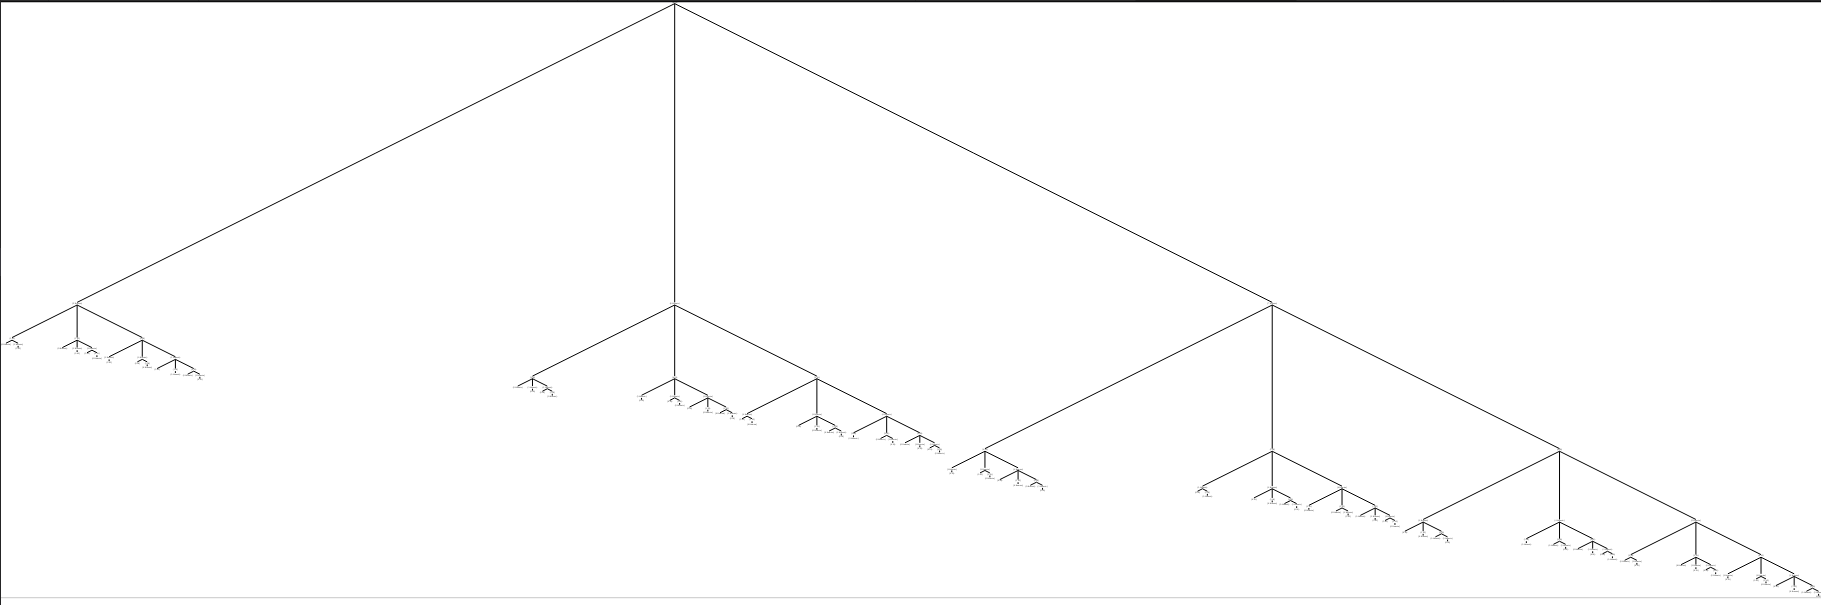
\includegraphics[scale = 0.25]{Arbre_latex.png}

\begin{inctext}
    
    \Tree [.{(8 IA)} 
    [.{(5 Humain)}  
        [.{(2  IA)} 
            {(0 Humain)} 
            [.{(1 Humain)} 
            {(0 IA)} ] ] 
        [.{(3 IA)} 
            {(0 Humain)} 
            [.{(1 Humain)} 
            {(0 IA)} ] 
            [ .{(2  Humain)} 
            {(0 IA)} 
            [.{(1 IA)} 
            {(0 Humain)} ] ]   ] 
            [.{(4 IA)}  
            [.{(1 Humain)} 
                {(0 IA)} ]  
            [ .{(2  Humain)} 
                {(0 IA)} 
                [.{(1 IA)} 
                    {(0 Humain)} ] ]  
                    [.{(3 Humain)} 
                {(0 IA)} 
                [.{(1 IA)} 
                {(0 Humain)} ] 
                [ .{(2  IA)} 
                {(0 Humain)} 
                [.{(1 Humain)} 
                {(0 IA)} ] ]  ] ]  ] 
                [.{(6 Humain)} 
                [.{(3 IA)} 
                {(0 Humain)} 
                [.{(1 Humain)} 
                {(0 IA)} ] 
                [ .{(2  Humain)}
                {(0 IA)} 
                [.{(1 IA)} 
                {(0 Humain)} ] ]   ] 
                [.{(4 IA)}  
                [.{(1 Humain)} 
                {(0 IA)} ]
                [ .{(2  Humain)} 
                {(0 IA)} 
                [.{(1 IA)} 
                {(0 Humain)} ] ]  
            [.{(3 Humain)} 
                {(0 IA)} 
                [.{(1 IA)} 
                    {(0 Humain)} ] 
                    [.{(2  IA)} 
                    {(0 Humain)} 
                    [.{(1 Humain)} 
                    {(0 IA)} ] ]  ] ] 
                    [.{(5 IA)}  
                    [ .{(2  Humain)} 
                    {(0 IA)} 
                    [.{(1 IA)} 
                    {(0 Humain)} ] ] 
                    [.{(3 Humain)} 
                    {(0 IA)} 
                    [.{(1 IA)} 
                    {(0 Humain)} ] 
                    [ .{(2  IA)} 
                    {(0 Humain)} 
                    [.{(1 Humain)} 
                    {(0 IA)} ] ]  ] 
                    [.{(4 Humain)}  
                    [.{(1 IA)} 
                    {(0 Humain)} ]   
                [.{(2  IA)} 
                    {(0 Humain)} 
                    [.{(1 Humain)} 
                            {(0 IA)} ] ]  
                            [.{(3 IA)} 
                    {(0 Humain)} 
                    [.{(1 Humain)} 
                    {(0 IA)} ] 
                    [ .{(2  Humain)} 
                    {(0 IA)} 
                    [.{(1 IA)} 
                            {(0 Humain)} ] ]   ] ]  ]  ] 
                            [.{(7 Humain)} 
                            [.{(4 IA)}  
                            [.{(1 Humain)} 
                            {(0 IA)} ] 
                            [ .{(2  Humain)} 
                            {(0 IA)} 
                            [.{(1 IA)} 
                            {(0 Humain)} ] ]  
                            [.{(3 Humain)} 
                            {(0 IA)} 
                            [.{(1 IA)} 
                            {(0 Humain)} ] 
                            [ .{(2  IA)} 
                            {(0 Humain)} 
                            [.{(1 Humain)} 
                            {(0 IA)} ] ]  ] ]  
    [.{(5 IA)}  
        [ .{(2  Humain)} 
            {(0 IA)} 
            [.{(1 IA)} 
            {(0 Humain)} ] ]
            [.{(3 Humain)} 
            {(0 IA)} 
            [.{(1 IA)} 
            {(0 Humain)} ] 
            [ .{(2  IA)} 
            {(0 Humain)} 
            [.{(1 Humain)} 
                    {(0 IA)} ] ]  ] 
        [.{(4 Humain)}  
            [.{(1 IA)} 
                {(0 Humain)} ]  
                [ .{(2  IA)} 
                {(0 Humain)} 
                [.{(1 Humain)} 
                    {(0 IA)} ] ]
                    [.{(3 IA)} {(0 Humain)} [.{(1 Humain)} {(0 IA)} ] [ .{(2  Humain)} {(0 IA)} [.{(1 IA)} {(0 Humain)} ] ]   ] ]  ]  
                    [.{(6 IA)} 
                    [.{(3 Humain)} 
                    {(0 IA)} 
                    [.{(1 IA)} 
                    {(0 Humain)} ] 
                    [ .{(2  IA)} 
                    {(0 Humain)} 
                    [.{(1 Humain)} 
                    {(0 IA)} ] ]  ] 
                    [.{(4 Humain)}  
                    [.{(1 IA)} 
                    {(0 Humain)} ] 
                    [.{(2  IA)} 
                    {(0 Humain)} 
                    [.{(1 Humain)} 
                    {(0 IA)} ] ]  
                    [.{(3 IA)} 
                    {(0 Humain)} 
                    [.{(1 Humain)} 
                    {(0 IA)} ] 
                    [ .{(2  Humain)} 
                    {(0 IA)} 
                    [.{(1 IA)} 
                    {(0 Humain)} ] ]   ] ] 
        [.{(5 Humain)}  
            [.{(2  IA)} 
            {(0 Humain)} 
            [.{(1 Humain)} 
            {(0 IA)} ] ] 
            [.{(3 IA)} 
                {(0 Humain)} 
                [.{(1 Humain)} 
                    {(0 IA)} ] 
                    [ .{(2  Humain)} 
                    {(0 IA)} 
                    [.{(1 IA)} 
                    {(0 Humain)} ] ]   ] 
                    [.{(4 IA)}  
                    [.{(1 Humain)} 
                    {(0 IA)} ]
                    [ .{(2  Humain)} 
                    {(0 IA)} 
                    [.{(1 IA)} 
                    {(0 Humain)} ] ]
                    [.{(3 Humain)} 
                    {(0 IA)} 
                    [.{(1 IA)} 
                        {(0 Humain)} ] 
                        [ .{(2  IA)} 
                        {(0 Humain)} 
                        [.{(1 Humain)} 
                        {(0 IA)} ] ]  ] ]  ]  ]  ]  ]
                        
                        
                    \end{inctext}
                    
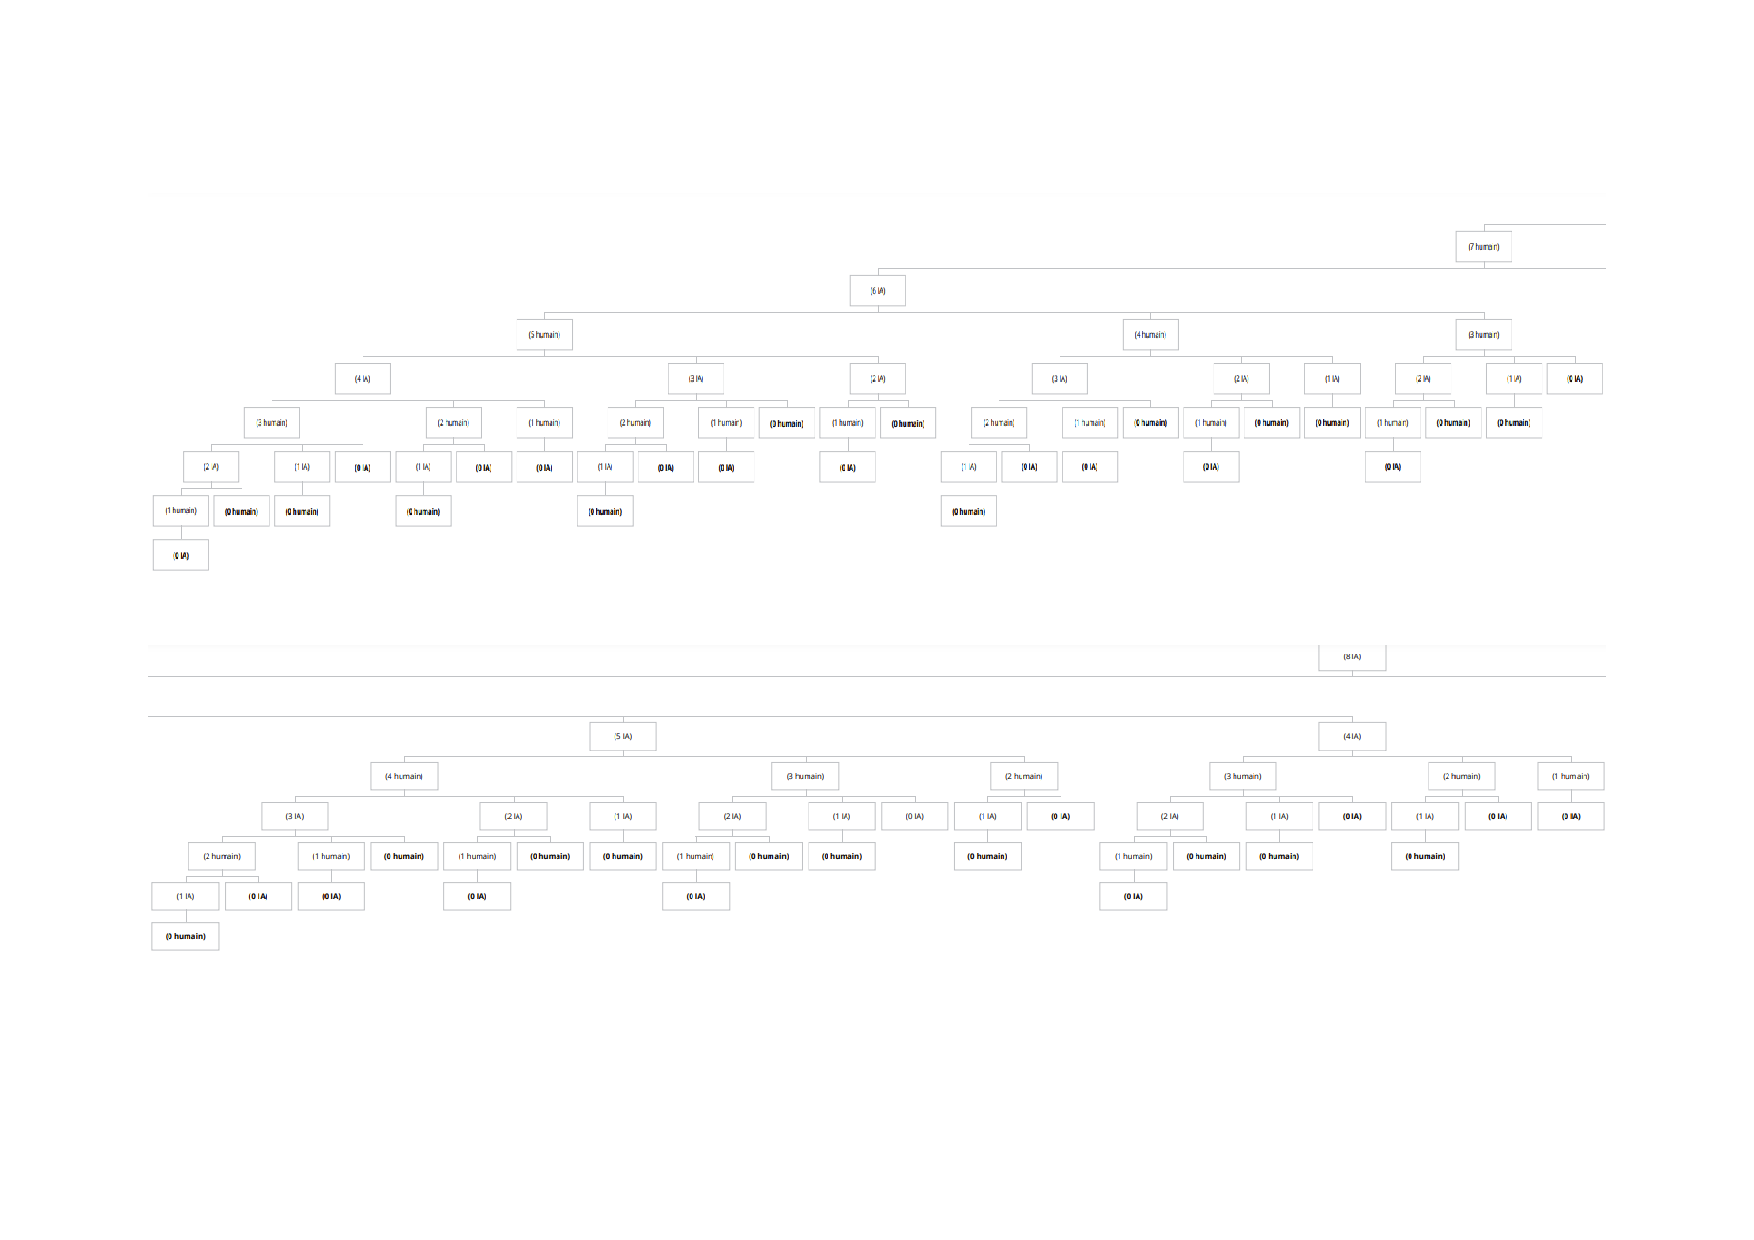
\includepdf[pages=-]{ArbreCamille.pdf}
                    
                    \begin{enumerate}
\def\labelenumi{\arabic{enumi}.}
\setcounter{enumi}{2}
\tightlist
\item
Explication du code :
\end{enumerate}

\begin{Shaded}
    \begin{algorithm}[H]
        \caption{Successeurs}
        \begin{Highlighting}[]
            
            \CommentTok{;; fonction qui donne tous les successeurs d\textquotesingle{}un état :}
            \NormalTok{(}\KeywordTok{defun}\FunctionTok{ successeurs }\NormalTok{(allumettes actions)}
            \NormalTok{  (}\KeywordTok{cdr}\NormalTok{ (}\KeywordTok{assoc}\NormalTok{ allumettes actions)))}
        \end{Highlighting}
\end{algorithm}
\end{Shaded}

\begin{Shaded}
    \begin{algorithm}[H]
        \caption{Explore}
\begin{Highlighting}[]
\CommentTok{;; EXPLORE }
\NormalTok{(}\KeywordTok{defun}\FunctionTok{ explore }\NormalTok{(allumettes actions joueur i)}
\NormalTok{  (}\KeywordTok{cond} 
\NormalTok{   ((}\KeywordTok{and}\NormalTok{ (}\KeywordTok{eq}\NormalTok{ joueur \textquotesingle{}humain) (}\KeywordTok{eq}\NormalTok{ allumettes }\DecValTok{0}\NormalTok{)) }\KeywordTok{nil}\NormalTok{) }
   \CommentTok{; Si le joueur est un humain et qu\textquotesingle{}il n\textquotesingle{}y a plus d\textquotesingle{}allumettes }
   \CommentTok{; sur la table, l\textquotesingle{}IA a perdu la partie.}
\NormalTok{   ((}\KeywordTok{and}\NormalTok{ (}\KeywordTok{eq}\NormalTok{ joueur \textquotesingle{}IA) (}\KeywordTok{eq}\NormalTok{ allumettes }\DecValTok{0}\NormalTok{)) }\KeywordTok{t}\NormalTok{)}
   \CommentTok{; Si le joueur est l\textquotesingle{}IA et qu\textquotesingle{}il n\textquotesingle{}y a plus d\textquotesingle{}allumettes sur la table, l\textquotesingle{}IA a gagné la partie.}
   \CommentTok{; Les deux conditions précédentes représentent les conditions d\textquotesingle{}arrêt de la récursivité.}
\NormalTok{    (}\KeywordTok{t}\NormalTok{ (}\KeywordTok{progn}                             
\NormalTok{         (}\KeywordTok{let}\NormalTok{ ((sol }\KeywordTok{nil}\NormalTok{) (coups (successeurs allumettes actions))) }
         \CommentTok{; Lorsque nous ne sommes pas dans les conditions d\textquotesingle{}arrêt décrites précédemment, on }
         \CommentTok{; initialise des variables locales sol et coups. Coups est une liste qui représente}
         \CommentTok{; l\textquotesingle{}ensemble des successeurs possibles de l\textquotesingle{}état courant et sol est une liste}
         \CommentTok{; initialement vide. sol permettra de stocker le chemin vers la solution si celle{-}ci}
         \CommentTok{; est trouvée lors du parcours. }
\NormalTok{           (while (}\KeywordTok{and}\NormalTok{ coups (}\KeywordTok{not}\NormalTok{ sol)) }
           \CommentTok{; On boucle tant qu\textquotesingle{}il reste des successeurs et que sol est nul.}
\NormalTok{             (}\KeywordTok{progn}
\NormalTok{               (}\KeywordTok{format} \KeywordTok{t} \StringTok{"\textasciitilde{}\%\textasciitilde{}V@tJoueur \textasciitilde{}s joue \textasciitilde{}s allumettes {-} il reste \textasciitilde{}s }
\StringTok{               allumette(s) "}\NormalTok{ i joueur (}\KeywordTok{car}\NormalTok{ coups) (}\OperatorTok{{-}}\NormalTok{ allumettes (}\KeywordTok{car}\NormalTok{ coups)))}
               \CommentTok{; On affiche le joueur courant, le nombre d\textquotesingle{}allumettes jouées et}
               \CommentTok{; le nombre d\textquotesingle{}allumettes restantes après le tirage.}
\NormalTok{                (}\KeywordTok{setq}\NormalTok{ sol (explore (}\OperatorTok{{-}}\NormalTok{ allumettes (}\KeywordTok{car}\NormalTok{ coups)) actions }
\NormalTok{                (}\KeywordTok{if}\NormalTok{ (}\KeywordTok{eq}\NormalTok{ joueur \textquotesingle{}IA) \textquotesingle{}humain \textquotesingle{}IA) (}\OperatorTok{+}\NormalTok{ i }\DecValTok{3}\NormalTok{)))}
                \CommentTok{; On rappelle la fonction explore avec le nombre d\textquotesingle{}allumettes }
                \CommentTok{; moins le nombre d\textquotesingle{}allumettes tirées, les actions possibles, }
                \CommentTok{; le joueur suivant et i + 3 afin d\textquotesingle{}indenter l\textquotesingle{}affichage. Le résultat }
                \CommentTok{; de l\textquotesingle{}appel de la fonction explore est stocké dans sol.}
\NormalTok{                (}\KeywordTok{if}\NormalTok{ sol           }
\NormalTok{                    (}\KeywordTok{setq}\NormalTok{ sol (}\KeywordTok{car}\NormalTok{ coups)))}
                \CommentTok{; Suite aux appels récursifs de la fonction explore, Si une }
                \CommentTok{; solution a été trouvée, sol prend la valeur du premier élément de coup}
\NormalTok{               (}\KeywordTok{format} \KeywordTok{t} \StringTok{"\textasciitilde{}\%\textasciitilde{}V@t sol = \textasciitilde{}s\textasciitilde{}\%"}\NormalTok{ i sol)}
               \CommentTok{; On affiche la solution trouvée}
\NormalTok{               (}\KeywordTok{pop}\NormalTok{ coups)}
               \CommentTok{;Suppression du premier élément de coups, permet de passer à l\textquotesingle{}élément}
               \CommentTok{; suivant de la liste de successeurs (incrémentation du while) }
\NormalTok{               ))  }
\NormalTok{           sol)))))   \CommentTok{; On retourne sol}}
\end{Highlighting}
\end{algorithm}
\end{Shaded}      
    

\begin{Shaded}
    \begin{algorithm}[H]
\begin{Highlighting}[]
\NormalTok{(}\KeywordTok{defvar}\FunctionTok{ nbCoupsAJouer }\KeywordTok{nil}\NormalTok{)}
\NormalTok{(}\KeywordTok{setq}\NormalTok{ nbCoupsAJouer (explore }\DecValTok{16}\NormalTok{ actions \textquotesingle{}IA }\DecValTok{0}\NormalTok{))}
\NormalTok{(}\KeywordTok{setq}\NormalTok{ nbCoupsAJouer (explore }\DecValTok{8}\NormalTok{ actions \textquotesingle{}IA }\DecValTok{0}\NormalTok{))}
\NormalTok{(}\KeywordTok{setq}\NormalTok{ nbCoupsAJouer (explore }\DecValTok{3}\NormalTok{ actions \textquotesingle{}IA }\DecValTok{0}\NormalTok{))}
\end{Highlighting}
\end{algorithm}
\end{Shaded}

La fonction regarde d'abord si on est dans un état final :
\begin{itemize}
    \item Si nous sommes dans un état final et que le joueur est l'IA alors on renvoie T 
    \item Si nous sommes dans un état final et que le joueur est l'humain alors on renvoie NIL.
\end{itemize}

Ensuite, on initialise la variable sol, qui indique si la solution a été
trouvée ou non. Cette variable est à nil tant qu'aucune solution n'a été
trouvée. De même, la variable coups est initialisée et elle prend tous
les successeurs de l'état en question, c'est à dire, renvoie le nombre
de coups possibles pour un nombre d'allumettes donné.\\
Tant qu'il reste des coups et que la solution n'a pas été trouvée, on
rappelle la fonction explore avec le nombre d'allumettes auquel on
retire le nombre de coups, les actions, et le joueur qui devient humain
si le joueur courant était IA et vice-versa.\\
Si la solution a été trouvée, on met sol au nombre de coups utilisé.\\
On passe au nombre de coups suivant.\\
On renvoie la solution.\\
Cet algorithme effectue donc une recherche en profondeur. En effet, un
parcours en largeur aurait exploré toutes les possibilités du niveau n+1
avant de passer aux états du niveau n+2.

En résumé, cette fonction explore permet de faire jouer chacun leur tour
l'IA et l'Humain grâce à un parcours en profondeur.

\begin{enumerate}
\def\labelenumi{\arabic{enumi}.}
\setcounter{enumi}{3}
\item
  Les deux solutions permettent de parvenir au résultat et de parcourir
  toutes les solutions.\\
  Pour effectuer un parcours en largeur il faudra tout de même penser à
  modifier la condition d'arrêt. Le parcous en profondeur a pour
  avantage de remonter facilement tous les chemins en les concaténant.
  Mais le parcours en largeur est notamment intéressant pour les graphes
  importants car il permet d'être plus rapide sur ce type de graphe, ce
  qui est le cas ici.
\item
  Il serait possible d'optimiser le parcours en utilisant une statégie
  bien connue du jeu de Nim. En effet, au jeu de Nim il est possible de
  toujours laisser un nombre d'allumettes multiples de 4 (4 8 12 16) sur
  la table afin de gagner plus souvent. Néanmoins, comme l'IA commence à
  jouer, elle n'est pas sûre de gagner à tous les coups car cette
  technique permet de gagner à tous les coups uniquement pour le 2eme
  joueur. Si le joueur en face utilise aussi cette stratégie, il sera
  donc impossible pour l'IA de gagner la partie.
\end{enumerate}

\pagebreak

\hypertarget{ruxe9solution-2-1}{%
\section{Résolution 2 :}\label{ruxe9solution-2-1}}

Dans cette seconde résolution, nous allons programmer une IA sans
stratégie du meilleur choix. Cette IA commencera le jeu et sera capable
d'améliorer sa stratégie face à un joueur humain.

\hypertarget{principe-de-lia}{%
\subsection{Principe de l'IA :}\label{principe-de-lia}}

Lorsque c'est son tour, cette IA choisira, au hasard parmi les
possibilités, un nombre d'allumettes à retirer. Une fois ce choix
réalisé, les allumettes seront retirées et le jeu passera au joueur
suivant.

A la fin de la partie, si l'IA gagne, elle voudra renforcer sa stratégie
gagnante. L'idée est d'ajouter le coup gagnant à la position qui a rendu
possible la victoire. Ce renforcement sera propagé aux positions qui ont
mené à cette victoire. Au prochain jeu, les probabilités de tomber sur
un coup qui mène à la victoire sont augmentées. Des stratégies gagnantes
devraient émerger.

\begin{enumerate}
\def\labelenumi{\arabic{enumi}.}
\setcounter{enumi}{1}
\tightlist
\item
  Fonction de lecture d'un coup que veut jouer l'utilisateur (humain) :
\end{enumerate}

\textbf{Spécification} : JeuJoueur (NbAllumettes, listeActions)\\
\emph{Entree} : 
\begin{itemize}
\item NbAllumettes correspond au nombre d'allumettes sur la
table.
\item listeActions correspond à la liste des actions possibles.
\end{itemize}
\emph{Sortie} : Entier lu au clavier compatible avec la liste
d'actions.\\
\emph{Objectif} : Cette fonction permet de lire au clavier un choix de
l'utilisateur. Elle vérifie si l'utilisateur rentre bien une valeur
comprise dans le spectre de valeur souhaité. Il faut donc que la valeur
entrée par l'utilisateur appartienne à une valeur possible dans la liste
actions.

Deux solutions ont été implémentées.
\begin{algorithm}[H]
\begin{Shaded}
\begin{Highlighting}[]
    \caption{JeuJoueur}
\NormalTok{(}\KeywordTok{defun}\FunctionTok{ JeuJoueur }\NormalTok{(NbAllumettes listeActions)}
\NormalTok{    (}\KeywordTok{let}\NormalTok{ ((lecture }\DecValTok{5}\NormalTok{)}
\NormalTok{        (possible (}\KeywordTok{assoc}\NormalTok{ NbAllumettes listeActions)))}
\NormalTok{        (while (}\KeywordTok{not}\NormalTok{ (}\KeywordTok{member}\NormalTok{ lecture (}\KeywordTok{cdr}\NormalTok{ possible)))}
\NormalTok{            (}\KeywordTok{format} \KeywordTok{t} \StringTok{"Rentrer le coup à jouer (il reste \textasciitilde{}s allumettes): \textasciitilde{}\&"}\NormalTok{ NbAllumettes)}
\NormalTok{            (}\KeywordTok{setq}\NormalTok{ lecture (}\KeywordTok{read}\NormalTok{))}
\NormalTok{        )}
\NormalTok{        lecture}
\NormalTok{    )}
\NormalTok{)       }
\end{Highlighting}
\end{Shaded}
\end{algorithm}

\begin{algorithm}[H]
\begin{Shaded}
\begin{Highlighting}[]
  \caption{JeuJoueur}
\NormalTok{(}\KeywordTok{defun}\FunctionTok{ JeuJoueur }\NormalTok{(allumettes actions)}
\NormalTok{  (}\KeywordTok{let}\NormalTok{ ((choix\_joueur }\KeywordTok{nil}\NormalTok{)}
\NormalTok{        (coups }\KeywordTok{nil}\NormalTok{))}
\NormalTok{    (while (}\KeywordTok{not}\NormalTok{ choix\_joueur)}
\NormalTok{      (}\KeywordTok{format} \KeywordTok{t} \StringTok{"Rentrer le coup à jouer (il reste \textasciitilde{}s allumettes): \textasciitilde{}\&"}\NormalTok{ allumettes)}
\NormalTok{      (}\KeywordTok{setq}\NormalTok{ coups (}\KeywordTok{read}\NormalTok{))}
\NormalTok{      (}\KeywordTok{setq}\NormalTok{ choix\_joueur (}\KeywordTok{member}\NormalTok{ coups (successeurs allumettes actions)))}
\NormalTok{      )}
\NormalTok{    coups)}
\NormalTok{  )}
\end{Highlighting}
\end{Shaded}
\end{algorithm}
Exemple d'execution :

\begin{Shaded}
    \begin{algorithm}[H]
\begin{Highlighting}[]
\OperatorTok{\textgreater{}}\NormalTok{ (JeuJoueur }\DecValTok{5}\NormalTok{ actions)}
\OperatorTok{\textgreater{}}\NormalTok{ Rentrer le coup à jouer (il reste }\DecValTok{5}\NormalTok{ allumettes) :}
\OperatorTok{\textgreater{}} \DecValTok{2}
\OperatorTok{\textgreater{}} \DecValTok{2}

\OperatorTok{\textgreater{}}\NormalTok{ (JeuJoueur }\DecValTok{8}\NormalTok{ actions)}
\OperatorTok{\textgreater{}}\NormalTok{ Rentrer le coup à jouer (il reste }\DecValTok{8}\NormalTok{ allumettes) :}
\OperatorTok{\textgreater{}} \DecValTok{5}
\OperatorTok{\textgreater{}}\NormalTok{ Rentrer le coup à jouer (il reste }\DecValTok{8}\NormalTok{ allumettes) :}
\OperatorTok{\textgreater{}} \DecValTok{1}
\OperatorTok{\textgreater{}} \DecValTok{1}

\OperatorTok{\textgreater{}}\NormalTok{ (JeuJoueur }\DecValTok{2}\NormalTok{ actions)}
\OperatorTok{\textgreater{}}\NormalTok{ Rentrer le coup à jouer (il reste }\DecValTok{2}\NormalTok{ allumettes) :}
\OperatorTok{\textgreater{}} \DecValTok{3}
\OperatorTok{\textgreater{}}\NormalTok{ Rentrer le coup à jouer (il reste }\DecValTok{2}\NormalTok{ allumettes):}
\OperatorTok{\textgreater{}} \DecValTok{2}
\OperatorTok{\textgreater{}} \DecValTok{2}
\end{Highlighting}
\end{algorithm}
\end{Shaded}

Nous avons trouvé deux implémentations de la fonction JeuJoueur. Ces
deux fonctions sont fonctionnelles. Néanmoins, nous avons préféré garder
dans la suite du TP la seconde version puisque celle-ci utilise la
fonction \emph{successeurs} que nous avons défini précédemment.

\pagebreak

\begin{enumerate}
\def\labelenumi{\arabic{enumi}.}
\setcounter{enumi}{2}
\tightlist
\item
  Algorithme de l'exploration renforcée :
\end{enumerate}

\textbf{Spécification} : explore-renf1 (nb\_allumettes, actions)\\
\emph{Entree} :
\begin{itemize}
\item nb\_allumettes correspond au nombre d'allumettes sur la table.
\item actions correspond à la liste des actions possibles
\end{itemize}

\emph{Sortie} : Renvoie la liste actions si l'IA gagne, nil sinon.\\
\emph{Objectif} : Cette fonction effectue l'exploration en profondeur
des possibilités du jeu de Nim.\\
Elle permet de faire jouer l'IA qui choisit un nombre d'allumettes à
retirer aléatoirement et le joueur qui lui peut entrer au clavier le
nombre d'allumettes qu'il souhaite retirer.

\begin{algorithm}[H]
    \caption{explore-renf1}
\begin{verbatim}
 explore-renf1 (nb_allumettes actions)
    IA_coups <- Nil
    humain_coups <- Nil
    Si nb_allumettes == 0 alors :
        Retourner actions
    Sinon si nb_allumettes == 1 alors :
        Retourner nil
    Sinon :
        IA_coups <- Randomsuccesseurs (successeurs (nb_allumettes, actions))     
        Affichage ("L'IA joue IA_coups")
        nb_allumettes <- nb_allumettes - IA_coups
        Si nb_allumettes > 0 alors :
            humain_coups <- JeuJoueur (nb_allumettes, actions)
            nb_allumettes <- nb_allumettes - humain_coups
            explore-renf1 (nb_allumettes, actions)
        Sinon :
            explore-renf1 (1, actions)
\end{verbatim}
\end{algorithm}


\begin{Shaded}    
    \begin{algorithm}[H]
        \caption{explore-renf1}
\begin{Highlighting}[]

\NormalTok{(}\KeywordTok{defun}\FunctionTok{ explore{-}renf1 }\NormalTok{(nb\_allumettes actions)}
\NormalTok{  (}\KeywordTok{let}\NormalTok{ ((IA\_coups) (humain\_coups))}
\NormalTok{    (}\KeywordTok{cond} 
\NormalTok{     ((}\OperatorTok{=}\NormalTok{ nb\_allumettes }\DecValTok{0}\NormalTok{) actions) }\CommentTok{;; IA gagne}
\NormalTok{     ((}\OperatorTok{=}\NormalTok{ nb\_allumettes }\DecValTok{1}\NormalTok{) }\KeywordTok{nil}\NormalTok{) }\CommentTok{;; IA perd}
\NormalTok{     (}\KeywordTok{t} \NormalTok{(}\KeywordTok{progn}\CommentTok{;; IA qui joue}
\NormalTok{            (}\KeywordTok{setq}\NormalTok{ IA\_coups (Randomsuccesseurs (successeurs nb\_allumettes actions)))}
\NormalTok{        (}\KeywordTok{format} \KeywordTok{t} \StringTok{"L\textquotesingle{}IA joue \textasciitilde{}s \textasciitilde{}\&"}\NormalTok{ IA\_coups)}
\NormalTok{            (}\KeywordTok{setq}\NormalTok{ nb\_allumettes (}\OperatorTok{{-}}\NormalTok{ nb\_allumettes IA\_coups))}
        \CommentTok{;; humain qui joue}
\NormalTok{        (}\KeywordTok{if}\NormalTok{ (}\OperatorTok{\textgreater{}}\NormalTok{ nb\_allumettes }\DecValTok{0}\NormalTok{)}
\NormalTok{            (}\KeywordTok{progn}
\NormalTok{            (}\KeywordTok{setq}\NormalTok{ humain\_coups (JeuJoueur nb\_allumettes actions))}
\NormalTok{              (}\KeywordTok{setq}\NormalTok{ nb\_allumettes (}\OperatorTok{{-}}\NormalTok{ nb\_allumettes humain\_coups))}
\NormalTok{            (explore{-}renf1 nb\_allumettes actions)}
\NormalTok{              )}
\NormalTok{          (explore{-}renf1 }\DecValTok{1}\NormalTok{ actions))}
\NormalTok{            )}
\NormalTok{        ))}
\NormalTok{    ))}
\end{Highlighting}
    \end{algorithm}
\end{Shaded}

Exemple d'execution :

\begin{Shaded}
    \begin{algorithm}[H]
\begin{Highlighting}[]
\OperatorTok{\textgreater{}}\NormalTok{ (explore{-}renf1 }\DecValTok{16}\NormalTok{ actions)}
\NormalTok{L\textquotesingle{}IA joue }\DecValTok{2} 
\NormalTok{Rentrer le coup à jouer (il reste }\DecValTok{14}\NormalTok{ allumettes): }
\DecValTok{2}
\NormalTok{L\textquotesingle{}IA joue }\DecValTok{3} 
\NormalTok{Rentrer le coup à jouer (il reste }\DecValTok{9}\NormalTok{ allumettes): }
\DecValTok{3}
\NormalTok{L\textquotesingle{}IA joue }\DecValTok{2} 
\NormalTok{Rentrer le coup à jouer (il reste }\DecValTok{4}\NormalTok{ allumettes): }
\DecValTok{1}
\NormalTok{L\textquotesingle{}IA joue }\DecValTok{1} 
\NormalTok{Rentrer le coup à jouer (il reste }\DecValTok{2}\NormalTok{ allumettes): }
\DecValTok{1}
\NormalTok{NIL}
\end{Highlighting}
\end{algorithm}
\end{Shaded}
\pagebreak
\begin{Shaded}
    \begin{algorithm}[H]
    \begin{Highlighting}[]
\OperatorTok{\textgreater{}}\NormalTok{ (explore{-}renf1 }\DecValTok{16}\NormalTok{ actions)}
\NormalTok{L\textquotesingle{}IA joue }\DecValTok{2} 
\NormalTok{Rentrer le coup à jouer (il reste }\DecValTok{14}\NormalTok{ allumettes): }
\DecValTok{3}
\NormalTok{L\textquotesingle{}IA joue }\DecValTok{2} 
\NormalTok{Rentrer le coup à jouer (il reste }\DecValTok{9}\NormalTok{ allumettes): }
\DecValTok{3}
\NormalTok{L\textquotesingle{}IA joue }\DecValTok{3} 
\NormalTok{Rentrer le coup à jouer (il reste }\DecValTok{3}\NormalTok{ allumettes): }
\DecValTok{3}
\NormalTok{((}\DecValTok{16} \DecValTok{3} \DecValTok{2} \DecValTok{1}\NormalTok{) (}\DecValTok{15} \DecValTok{3} \DecValTok{2} \DecValTok{1}\NormalTok{) (}\DecValTok{14} \DecValTok{3} \DecValTok{2} \DecValTok{1}\NormalTok{) (}\DecValTok{13} \DecValTok{3} \DecValTok{2} \DecValTok{1}\NormalTok{) (}\DecValTok{12} \DecValTok{3} \DecValTok{2} \DecValTok{1}\NormalTok{)}
\NormalTok{ (}\DecValTok{11} \DecValTok{3} \DecValTok{2} \DecValTok{1}\NormalTok{) (}\DecValTok{10} \DecValTok{3} \DecValTok{2} \DecValTok{1}\NormalTok{) (}\DecValTok{9} \DecValTok{3} \DecValTok{2} \DecValTok{1}\NormalTok{) (}\DecValTok{8} \DecValTok{3} \DecValTok{2} \DecValTok{1}\NormalTok{) (}\DecValTok{7} \DecValTok{3} \DecValTok{2} \DecValTok{1}\NormalTok{) ...)}
\end{Highlighting}
\end{algorithm}
\end{Shaded}

\begin{enumerate}
\def\labelenumi{\arabic{enumi}.}
\setcounter{enumi}{3}
\tightlist
\item
  Amélioration de l'algorithme précédent afin de le renforcer avec des
  stratégies déjà rencontrées comme décrite dans l'étape 9:
\end{enumerate}

\textbf{Spécification} : explore-renfDernierCoup (nb\_allumettes,
actions)\\
\emph{Entree} :
\begin{itemize}
\item nb\_allumettes correspond au nombre d'allumettes sur la table.
\item actions correspond à la liste des actions possibles.
\end{itemize}

\emph{Sortie} : la liste actions si l'IA gagne, nil sinon.\\
\emph{Objectif} : Cette fonction effectue l'exploration en profondeur
des possibilités du jeu de Nim.\\
Elle permet de faire jouer l'IA qui choisit un nombre d'allumettes à
retirer aléatoirement et le joueur qui lui peut entrer au clavier le
nombre d'allumettes qu'il souhaite retirer.\\
Si l'IA gagne, son dernier coup joué est ajouté à la sous-liste
correspondante de actions grace à la fonction \emph{renforcement.}
\begin{algorithm}[H]
    \caption{explore-renfDernierCoup}
\begin{verbatim}

explore-renfDernierCoup (nb_allumettes, actions)
    IA_coups <- Nil
    humain_coups <- Nil
    Si nb_allumettes == 0 alors :
        Retourner actions
    Sinon si nb_allumettes == 1 alors :
        Retourner nil
    Sinon :
        IA_coups <- Randomsuccesseurs (successeurs(nb_allumettes, actions))
        Affichage ("L'IA joue IA_coups")
        dernier_coup <- Liste(nb_allumettes, IA_coups)
        nb_allumettes <- nb_allumettes - IA_coups
        Si nb_allumettes > 0 alors :
            humain_coups <- JeuJoueur (nb_allumettes, actions)
            nb_allumettes <- nb_allumettes - humain_coups
            Si nb_allumettes == 0 alors:
                Effectuer le renforcement de dernier_coup
            explore-renfDernierCoup (nb_allumettes, actions)
        Sinon :
            explore-renfDernierCoup (1, actions)
    \end{verbatim}
\end{algorithm}

\begin{Shaded}
\begin{algorithm}[H]
    \caption{explore-renfDernierCoup}
\begin{Highlighting}[]
\NormalTok{(}\KeywordTok{defun}\FunctionTok{ explore{-}renfDernierCoup }\NormalTok{(nb\_allumettes actions)}
\NormalTok{  (}\KeywordTok{let}\NormalTok{ ((IA\_coups ) (humain\_coups))}
\NormalTok{    (}\KeywordTok{cond} 
\NormalTok{     ((}\OperatorTok{=}\NormalTok{ nb\_allumettes }\DecValTok{0}\NormalTok{) actions) }\CommentTok{;; IA gagne}
\NormalTok{     ((}\OperatorTok{=}\NormalTok{ nb\_allumettes }\DecValTok{1}\NormalTok{) }\KeywordTok{nil}\NormalTok{) }\CommentTok{;; IA perd}
\NormalTok{     (}\KeywordTok{t} \NormalTok{(}\KeywordTok{progn}\CommentTok{;; IA qui joue}
\NormalTok{        (}\KeywordTok{setq}\NormalTok{ IA\_coups (Randomsuccesseurs (successeurs nb\_allumettes actions)))}
\NormalTok{        (}\KeywordTok{format} \KeywordTok{t} \StringTok{"L\textquotesingle{}IA joue \textasciitilde{}s \textasciitilde{}\&"}\NormalTok{ IA\_coups)}
\NormalTok{        (}\KeywordTok{setq}\NormalTok{ dernier\_coup (}\KeywordTok{list}\NormalTok{ nb\_allumettes IA\_coups))} 
\NormalTok{        (}\KeywordTok{setq}\NormalTok{ nb\_allumettes\_IA nb\_allumettes)}
\NormalTok{        (}\KeywordTok{setq}\NormalTok{ nb\_allumettes (}\OperatorTok{{-}}\NormalTok{ nb\_allumettes IA\_coups))}
        \CommentTok{;; humain qui joue}
\NormalTok{        (}\KeywordTok{if}\NormalTok{ (}\OperatorTok{\textgreater{}}\NormalTok{ nb\_allumettes }\DecValTok{0}\NormalTok{)}
\NormalTok{            (}\KeywordTok{progn}
\NormalTok{            (}\KeywordTok{setq}\NormalTok{ humain\_coups (JeuJoueur nb\_allumettes actions))}
\NormalTok{              (}\KeywordTok{setq}\NormalTok{ nb\_allumettes (}\OperatorTok{{-}}\NormalTok{ nb\_allumettes humain\_coups))}
\NormalTok{              (}\KeywordTok{when}\NormalTok{ (}\OperatorTok{=}\NormalTok{ nb\_allumettes }\DecValTok{0}\NormalTok{) }
\NormalTok{                  (renforcement nb\_allumettes\_IA IA\_coups actions)}
\NormalTok{              )}
\NormalTok{            (explore{-}renfDernierCoup nb\_allumettes actions)}
\NormalTok{            )}
\NormalTok{          (explore{-}renfDernierCoup }\DecValTok{1}\NormalTok{ actions))}
\NormalTok{        )))))}
\end{Highlighting}
\end{algorithm}
\end{Shaded}

Exemple d'execution :

\begin{Shaded}
    \begin{algorithm}[H]
\begin{Highlighting}[]
\OperatorTok{\textgreater{}}\NormalTok{ (explore{-}renfDernierCoup }\DecValTok{16}\NormalTok{ actions)}
\NormalTok{L\textquotesingle{}IA joue }\DecValTok{2} 
\NormalTok{Rentrer le coup à jouer (il reste }\DecValTok{14}\NormalTok{ allumettes): }
\DecValTok{3}
\NormalTok{L\textquotesingle{}IA joue }\DecValTok{3} 
\NormalTok{Rentrer le coup à jouer (il reste }\DecValTok{8}\NormalTok{ allumettes): }
\DecValTok{2}
\NormalTok{L\textquotesingle{}IA joue }\DecValTok{2} 
\NormalTok{Rentrer le coup à jouer (il reste }\DecValTok{4}\NormalTok{ allumettes): }
\DecValTok{1}
\NormalTok{L\textquotesingle{}IA joue }\DecValTok{3} 
\NormalTok{NIL}
\end{Highlighting}
\end{algorithm}
\end{Shaded}


\begin{Shaded}
    \begin{algorithm}[H]
    \begin{Highlighting}[]
\OperatorTok{\textgreater{}}\NormalTok{ (explore{-}renfDernierCoup }\DecValTok{16}\NormalTok{ actions)}
\NormalTok{L\textquotesingle{}IA joue }\DecValTok{2} 
\NormalTok{Rentrer le coup à jouer (il reste }\DecValTok{14}\NormalTok{ allumettes): }
\DecValTok{2}
\NormalTok{L\textquotesingle{}IA joue }\DecValTok{1} 
\NormalTok{Rentrer le coup à jouer (il reste }\DecValTok{11}\NormalTok{ allumettes): }
\DecValTok{2}
\NormalTok{L\textquotesingle{}IA joue }\DecValTok{1} 
\NormalTok{Rentrer le coup à jouer (il reste }\DecValTok{8}\NormalTok{ allumettes): }
\DecValTok{3}
\NormalTok{L\textquotesingle{}IA joue }\DecValTok{3} 
\NormalTok{Rentrer le coup à jouer (il reste }\DecValTok{2}\NormalTok{ allumettes): }
\DecValTok{2}
\NormalTok{((}\DecValTok{16} \DecValTok{3} \DecValTok{2} \DecValTok{1}\NormalTok{) (}\DecValTok{15} \DecValTok{3} \DecValTok{2} \DecValTok{1}\NormalTok{) (}\DecValTok{14} \DecValTok{3} \DecValTok{2} \DecValTok{1}\NormalTok{) (}\DecValTok{13} \DecValTok{3} \DecValTok{2} \DecValTok{1}\NormalTok{) (}\DecValTok{12} \DecValTok{3} \DecValTok{2} \DecValTok{1}\NormalTok{)}
\NormalTok{ (}\DecValTok{11} \DecValTok{3} \DecValTok{2} \DecValTok{1}\NormalTok{) (}\DecValTok{10} \DecValTok{3} \DecValTok{2} \DecValTok{1}\NormalTok{) (}\DecValTok{9} \DecValTok{3} \DecValTok{2} \DecValTok{1}\NormalTok{) (}\DecValTok{8} \DecValTok{3} \DecValTok{2} \DecValTok{1}\NormalTok{) (}\DecValTok{7} \DecValTok{3} \DecValTok{2} \DecValTok{1}\NormalTok{) ...)}
\end{Highlighting}
\end{algorithm}
\end{Shaded}

\begin{Shaded}
    \begin{algorithm}[H]
    \begin{Highlighting}[]
\CommentTok{;;vérification}
\OperatorTok{\textgreater{}}\NormalTok{ (successeurs }\DecValTok{5}\NormalTok{ actions)}
\NormalTok{(}\DecValTok{3} \DecValTok{2} \DecValTok{1} \DecValTok{3}\NormalTok{)}
\end{Highlighting}
\end{algorithm}
\end{Shaded}


\begin{enumerate}
\def\labelenumi{\arabic{enumi}.}
\setcounter{enumi}{4}
\tightlist
\item
  Pour cette question, nous avons implémenté une fonction lisp qui
  permet d'ajouter le coup gagnant aux coups possibles pour le nombre
  d'allumettes en jeu dans la liste actions.
\end{enumerate}

\textbf{Spécification} : renforcement (nbAllumettes, coup, actions)\\
\emph{Entree} :
\begin{itemize}
\item nbAllumettes correspond au nombre d'allumettes sur la table à
renforcer. 
\item coup correspond au coup à insérer dans la liste actions. 
\item actions correspond à la liste de toutes les actions possibles.
\end{itemize}

\emph{Sortie} : liste actions modifiée avec le coup donné en paramètre,
ajouté dans la sous-liste correspondante au nombre d'allumettes
nbAllumettes.\\
\emph{Objectif} : Cette fonction permet d'ajouter le coup gagnant aux
coups possibles pour le nombre d'allumettes en jeu dans la liste
actions.

\pagebreak
Deux fonctions ont été implémentées :

\begin{Shaded}
    \begin{algorithm}[H]
        \caption{renforcement}
\begin{Highlighting}[]
\NormalTok{(}\KeywordTok{defun}\FunctionTok{ renforcement }\NormalTok{(nbAllumettes coup actions)}
\NormalTok{    (}\KeywordTok{let}\NormalTok{ ((toAdd (}\KeywordTok{append}\NormalTok{ (}\KeywordTok{list}\NormalTok{ nbAllumettes coup) }\NormalTok{(}\KeywordTok{cdr}\NormalTok{ (}\KeywordTok{assoc}\NormalTok{ nbAllumettes actions)))))}
    \CommentTok{; On prépare l\textquotesingle{}element a ajouter (liste composée du nombre d\textquotesingle{}allumettes,}
    \CommentTok{; du coup et des autres possibilitées déjà présentes dans actions)}
\NormalTok{    (}\KeywordTok{setf}\NormalTok{ (}\KeywordTok{nth}\NormalTok{  (}\OperatorTok{*}\NormalTok{ (}\OperatorTok{{-}}\NormalTok{ nbAllumettes }\DecValTok{16}\NormalTok{) }\DecValTok{{-}1}\NormalTok{) actions) toAdd)}
    \CommentTok{; On récupère l\textquotesingle{}indice ou se trouve la sous-liste correspondante au nombre d\textquotesingle{}allumettes}
    \CommentTok{; et on la modifie grâce au setf par la sous-liste toAdd cree précédement.}
\NormalTok{    actions))}\CommentTok{; On retourne actions}
\end{Highlighting}
\end{algorithm}
\end{Shaded}

\begin{Shaded}
    \begin{algorithm}[H]
        \caption{renforcement}
\begin{Highlighting}[]
\NormalTok{(}\KeywordTok{defun}\FunctionTok{ renforcement }\NormalTok{(nbAllumettes coup actions)}
\NormalTok{  (}\KeywordTok{setf}\NormalTok{ (}\KeywordTok{cdr}\NormalTok{ (}\KeywordTok{assoc}\NormalTok{ nbAllumettes actions))}
\NormalTok{    (}\KeywordTok{nconc}\NormalTok{ (}\KeywordTok{cdr}\NormalTok{(}\KeywordTok{assoc}\NormalTok{ nbAllumettes actions)) (}\KeywordTok{list}\NormalTok{ coup)))}
\NormalTok{    actions)}
\end{Highlighting}
\end{algorithm}
\end{Shaded}

Exemple d'exécution :

\begin{Shaded}
    \begin{algorithm}[H]
\begin{Highlighting}[]
\NormalTok{(Renforcement }\DecValTok{7} \DecValTok{1}\NormalTok{ actions) {-}\textgreater{} (... (}\DecValTok{7} \DecValTok{3} \DecValTok{2} \DecValTok{1} \DecValTok{1}\NormalTok{) ...)}
\NormalTok{(Renforcement }\DecValTok{16} \DecValTok{3}\NormalTok{ actions) {-}\textgreater{} ((}\DecValTok{16} \DecValTok{3} \DecValTok{2} \DecValTok{1} \DecValTok{3}\NormalTok{) ...)}
\end{Highlighting}
\end{algorithm}
\end{Shaded}


\textbf{Explication} : Les deux fonctions utilisent un setf afin
d'accéder à la mémoire et de changer l'élément voulu. Dans la première
fonction l'accès se fait grace à l'indice de l'emplacement de la
sous-fonction d'actions correspondant à nbAllumettes. La deuxième
accède à la mémoire grâce à un cdr. Ainsi, la deuxième fonction reste
plus simple. En effet, elle permet de modifier la liste actions sans
calculer l'indice de la sous-liste correspondante. C'est donc cette
fonction que l'on gardera pour la suite.

\begin{enumerate}
\def\labelenumi{\arabic{enumi}.}
\setcounter{enumi}{5}
\tightlist
\item
  Dans cette dernière partie, nous allons implémenter une fonction qui
  permet de renforcer l'IA avec tous les coups qu'elle a pu jouer dès
  qu'elle gagne la partie.
\end{enumerate}

\textbf{Spécification} : explore-renf-rec (nb\_allumettes, actions)\\
\emph{Entree} :
\begin{itemize}
\item nb\_allumettes correspond au nombre d'allumettes sur la table. 
\item actions correspond à la liste de toutes les actions possibles.
\end{itemize}

\emph{Sortie} : liste actions modifiée suite au renforcement si l'IA
gagne, nil sinon.\\
\emph{Objectif} : Sur le même principe que explore-renf1 (cf question
3), explore-renf-rec simule une partie de jeu de Nim.\\
Une liste a\_renf enregistre tous les coups de l'IA. Si elle gagne cette
liste est parcourue pour être utilisée dans la fonction renforcement
(definie à la question 5).

\textbf{Commentaire} : A part l'étape du renforcement décrite ci-dessus,
explore-renf fonctionne de la même manière que explore-renf1.\\
De plus, nous utilisons la fonction explore-renf-rec durant l'appel afin
de remettre à Nil la variable globale a\_renf.

\begin{algorithm}[H]
    \caption{explore-renf-rec}
\begin{verbatim}
explore-renf-rec (nb_allumettes, action)
  a_renf <- nil //(variable globale)
  explore-renf(nb_allumettes, actions)
\end{verbatim}
\end{algorithm}

\begin{algorithm}[H]
    \caption{explore-renf}
\begin{verbatim}
 explore-renf (nb_allumettes actions)
    IA_coups <- Nil
    humain_coups <- Nil
    Si nb_allumettes == 0 alors :
        Pour tout élément x de a_renf faire :
            renforcement de x
        Retourner a_renf
    Sinon si nb_allumettes == 1 alors:
        Retourner nil
    Sinon
        IA_coups <- Randomsuccesseurs (successeurs(nb_allumettes, actions))
        Affichage ("L'IA joue IA_coups")
        Ajouter dans a_renf la liste (IA_coups, nb_allumettes)
        nb_allumettes <- nb_allumettes - IA_coups
        Si nb_allumettes > 0 alors :
            humain_coups <- JeuJoueur (nb_allumettes, actions)
            nb_allumettes <- nb_allumettes - humain_coups
            explore-renf (nb_allumettes, actions)
        Sinon :
            explore-renf (1, actions)
\end{verbatim}
\end{algorithm}

\begin{Shaded}
    \begin{algorithm}[H]
    \caption{explore-renf-rec}
\begin{Highlighting}[]
\NormalTok{(}\KeywordTok{defun}\FunctionTok{ explore{-}renf{-}rec }\NormalTok{(nb\_allumettes actions)}
\NormalTok{  (}\KeywordTok{defparameter}\FunctionTok{ a}\NormalTok{\_renf }\KeywordTok{nil}\NormalTok{)}
\NormalTok{    (explore{-}renf nb\_allumettes actions))}
\end{Highlighting}
\end{algorithm}
\end{Shaded}

\begin{Shaded}
    \begin{algorithm}[H]
    \caption{explore-renf}
    \begin{Highlighting}[]
\NormalTok{(}\KeywordTok{defun}\FunctionTok{ explore{-}renf }\NormalTok{(nb\_allumettes actions)}
\NormalTok{  (}\KeywordTok{let}\NormalTok{ ((IA\_coups ) (humain\_coups))}
\NormalTok{    (}\KeywordTok{cond} 
\NormalTok{     ((}\OperatorTok{=}\NormalTok{ nb\_allumettes }\DecValTok{0}\NormalTok{) }
\NormalTok{        (}\KeywordTok{dolist}\NormalTok{ (x a\_renf actions)}
\NormalTok{          (renforcement (}\KeywordTok{car}\NormalTok{ x) (}\KeywordTok{cadr}\NormalTok{ x) actions)))} \CommentTok{;; IA gagne}
\NormalTok{     ((}\OperatorTok{=}\NormalTok{ nb\_allumettes }\DecValTok{1}\NormalTok{) }\KeywordTok{nil}\NormalTok{) }\CommentTok{;; IA perd}
\NormalTok{     (}\KeywordTok{t} \NormalTok{(}\KeywordTok{progn}\CommentTok{;; IA qui joue}  
\NormalTok{            (}\KeywordTok{setq}\NormalTok{ IA\_coups (Randomsuccesseurs (successeurs nb\_allumettes actions)))}
\NormalTok{            (}\KeywordTok{format} \KeywordTok{t} \StringTok{"L\textquotesingle{}IA joue \textasciitilde{}s \textasciitilde{}\&"}\NormalTok{ IA\_coups)}
\NormalTok{            (}\KeywordTok{push}\NormalTok{ (}\KeywordTok{list}\NormalTok{ nb\_allumettes IA\_coups) a\_renf)}
\NormalTok{            (}\KeywordTok{setq}\NormalTok{ nb\_allumettes (}\OperatorTok{{-}}\NormalTok{ nb\_allumettes IA\_coups))} 
\NormalTok{        (}\KeywordTok{if}\NormalTok{ (}\OperatorTok{\textgreater{}}\NormalTok{ nb\_allumettes }\DecValTok{0}\NormalTok{)}\CommentTok{;; humain qui joue}
\NormalTok{            (}\KeywordTok{progn}
\NormalTok{            (}\KeywordTok{setq}\NormalTok{ humain\_coups (JeuJoueur nb\_allumettes actions))}
\NormalTok{            (}\KeywordTok{setq}\NormalTok{ nb\_allumettes (}\OperatorTok{{-}}\NormalTok{ nb\_allumettes humain\_coups))}
\NormalTok{            (explore{-}renf nb\_allumettes actions)}
\NormalTok{              )}
\NormalTok{          (explore{-}renf }\DecValTok{1}\NormalTok{ actions)))))))}
\end{Highlighting}
\end{algorithm}
\end{Shaded}

Exemple d'exécution :

\begin{Shaded}
    \begin{algorithm}[H]
\begin{Highlighting}[]
\OperatorTok{\textgreater{}}\NormalTok{ (explore{-}renf{-}rec }\DecValTok{16}\NormalTok{ actions)}
\NormalTok{L\textquotesingle{}IA joue }\DecValTok{3} 
\NormalTok{Rentrer le coup à jouer (il reste }\DecValTok{13}\NormalTok{ allumettes): }
\DecValTok{2}
\NormalTok{L\textquotesingle{}IA joue }\DecValTok{1} 
\NormalTok{Rentrer le coup à jouer (il reste }\DecValTok{10}\NormalTok{ allumettes): }
\DecValTok{1}
\NormalTok{L\textquotesingle{}IA joue }\DecValTok{1} 
\NormalTok{Rentrer le coup à jouer (il reste }\DecValTok{8}\NormalTok{ allumettes): }
\DecValTok{3}
\NormalTok{L\textquotesingle{}IA joue }\DecValTok{2} 
\NormalTok{Rentrer le coup à jouer (il reste }\DecValTok{3}\NormalTok{ allumettes): }
\DecValTok{2}
\NormalTok{NIL}
\end{Highlighting}
\end{algorithm}
\end{Shaded}

\begin{Shaded}
    \begin{algorithm}[H]
\begin{Highlighting}[]
\OperatorTok{\textgreater{}}\NormalTok{ (explore{-}renf{-}rec }\DecValTok{16}\NormalTok{ actions)}
\NormalTok{L\textquotesingle{}IA joue }\DecValTok{2} 
\NormalTok{Rentrer le coup à jouer (il reste }\DecValTok{14}\NormalTok{ allumettes): }
\DecValTok{1}
\NormalTok{L\textquotesingle{}IA joue }\DecValTok{2} 
\NormalTok{Rentrer le coup à jouer (il reste }\DecValTok{11}\NormalTok{ allumettes): }
\DecValTok{3}
\NormalTok{L\textquotesingle{}IA joue }\DecValTok{1} 
\NormalTok{Rentrer le coup à jouer (il reste }\DecValTok{7}\NormalTok{ allumettes): }
\DecValTok{2}
\NormalTok{L\textquotesingle{}IA joue }\DecValTok{3} 
\NormalTok{Rentrer le coup à jouer (il reste }\DecValTok{2}\NormalTok{ allumettes): }
\DecValTok{2}
\NormalTok{((}\DecValTok{16} \DecValTok{3} \DecValTok{2} \DecValTok{1} \DecValTok{2}\NormalTok{) (}\DecValTok{15} \DecValTok{3} \DecValTok{2} \DecValTok{1}\NormalTok{) (}\DecValTok{14} \DecValTok{3} \DecValTok{2} \DecValTok{1}\NormalTok{) (}\DecValTok{13} \DecValTok{3} \DecValTok{2} \DecValTok{1} \DecValTok{2}\NormalTok{)}
\NormalTok{ (}\DecValTok{12} \DecValTok{3} \DecValTok{2} \DecValTok{1}\NormalTok{) (}\DecValTok{11} \DecValTok{3} \DecValTok{2} \DecValTok{1}\NormalTok{) (}\DecValTok{10} \DecValTok{3} \DecValTok{2} \DecValTok{1}\NormalTok{) (}\DecValTok{9} \DecValTok{3} \DecValTok{2} \DecValTok{1}\NormalTok{) (}\DecValTok{8} \DecValTok{3} \DecValTok{2} \DecValTok{1} \DecValTok{1}\NormalTok{)}
\NormalTok{ (}\DecValTok{7} \DecValTok{3} \DecValTok{2} \DecValTok{1}\NormalTok{) ...)}
\end{Highlighting}
\end{algorithm}
\end{Shaded}

\textbf{Explication} : La fonction explore-renf-rec définit une variable
globale a\_renf puis fait appel à la fonction explore-renf. Ainsi,
a\_renf sera reconnue dans explore-renf et sera remise à nil à chaque
appel de explore-renf-rec.\\
Pour procéder au renforcement des coups de l'IA, nous enregistrons dans
a\_renf chaque coup réalisé par l'IA avec son nombre d'allumettes
associés. La variable a\_renf étant globale, elle peut être réutilisée à
chaque appel récursif de explore-renf. Ainsi, lorsque l'IA gagne
(condition nb\_allumettes = 0) cette liste est parcourue pour pouvoir
renforcer la stratégie de l'IA.

\pagebreak

\hypertarget{conclusion}{%
\section{Conclusion}\label{conclusion}}

Lors de ce TP, nous avons eu l'occasion de tester deux résolutions
différentes du jeu de Nim. La première résolution constitue une
résolution naïve alors que lors de la seconde résolution, l'IA se
renforce et s'améliore au fil des parties.

Après plusieurs essais des deux résolutions, nous avons remarqué qu'au
début les deux résolutions sont équivalentes. Néanmoins, au bout d'un
certain nombre de parties, la seconde résolution devient beaucoup plus
efficace car l'IA applique des choix qui lui permettent de gagner grâce
aux parties précédentes qui ont renforcé sa stratégie. Lors de la
première partie les deux résolutions sont donc similaires mais au bout d'un
grand nombre de partie, l'IA de la seconde résolution devient beaucoup
plus forte alors que l'IA de la première résolution garde le même
niveau.

\end{document}
